\documentclass[12pt, letterpaper]{article}
\usepackage{graphicx} % Required for inserting images
\usepackage{hyperref}
\usepackage{listings}
\usepackage{amssymb}
\usepackage{amsmath}
\usepackage[english]{babel}
\usepackage{nicefrac, xfrac}
\usepackage{mathtools}
\usepackage[table,xcdraw]{xcolor}
\definecolor{light-gray}{gray}{0.95}
\definecolor{sap}{RGB}{130, 36, 51}
\definecolor{lg}{RGB}{102, 161, 95}
\definecolor{g}{RGB}{60, 50, 50}
\usepackage[paper=a4paper,left=20mm,right=20mm,bottom=25mm,top=25mm]{geometry}
\newcommand{\code}[1]{\colorbox{light-gray}{\texttt{#1}}}
\newcommand{\shelll}[1]{\colorbox{black}{\textcolor{white}{\texttt{#1}}}}
\newcommand{\shell}[1]{\colorbox{black}{\textcolor{white}{\texttt{casufrost@debian:$\sim$\$ #1}}}}
\newcommand{\codee}[1]{\colorbox{white}{\texttt{#1}}}
\newcommand{\acc}{\\\hphantom{}\\}
\newcommand{\dete}{{\rightarrow}}
\newcommand{\fdot}{{\(\bullet\) }}
\newcommand{\textg}[1]{\color{g}{\textbf{#1}}\color{black}}
\newcommand{\boxedMath}[1]{\begin{tabular}{|c|}\hline \texttt{#1} \\ \hline\end{tabular} :}
\title{Reti di Elaboratori}
\author{Marco Casu}
\date{\vspace{-5ex}}
\begin{document}



\maketitle
\begin{figure}[h]
    \centering{
    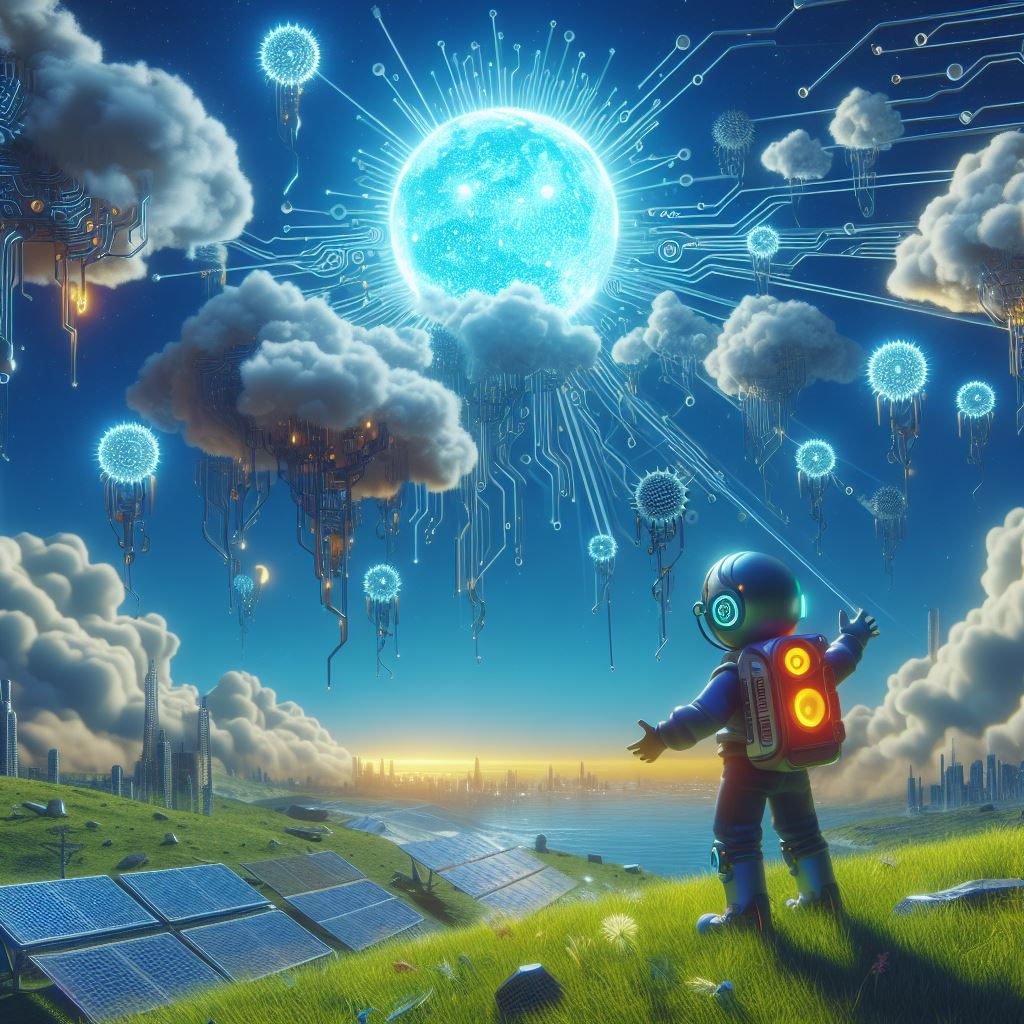
\includegraphics[width=1\textwidth ]{images/cop.jpg}
    }
\end{figure}
\newpage 
\tableofcontents
\newpage
\section{Reti di Calcolatori e Internet}
Cos'è una richiesta di rete? E soprattutto quali sono i passaggi ed il procedimento scaturito a seguito di una richiesta? Questo corso 
si concentrerà sull'aspetto del \textit{networking}, ossia, su come avviene la comunicazione tramite più elaboratori.\acc 
Una \textit{connessione} è una comunicazione aperta in cui sono coinvolte entrambe le parti in attesa di ricevere ed inviare 
messaggi, tramite l'apertura di un \textit{socket} (si approfondirà in seguito). Il problema di una comunicazione di questo tipo, 
è il bisogno di avere la certezza che i messaggi inviati da una parte siano ricevuti correttamente dall'altra, senza il rischio di 
comunicare "a vuoto", per questo sono definiti degli appositi protocolli.\acc 
\textbf{Host} : Un dispositivo connesso alla rete in modo periferico, non funge da esclusivo tramite per la comunicazione, 
ed è un sistema "periferico", esegue delle \textit{app} che forniscono servizi sulla rete.\acc 
\textbf{Switch} : Gli switch sono i dispositivi capaci di "instradare" i \textit{pacchetti}.\acc
\textbf{Rete} : Una collezione di dispositivi host/switch e collegamenti gestiti da un unico ente/organizzazione.\begin{center}
    \includegraphics[width=1\textwidth ]{images/reteDef.eps}
\end{center}
Quella che noi chiamiamo \textbf{internet}, è una "\textit{rete di reti}", ossia l'insieme interconnesso di tutte le reti 
pubbliche, che si stabilisce e necessita di protocolli su tutti i livelli : \begin{itemize}
    \item Livello di applicazione
    \item Livello di trasporto 
    \item Livello network 
    \item Livello di collegamento
\end{itemize}
Lo scopo di internet è quello di essere un infrastruttura che fornisce i servizi alle applicazioni distribuite, è 
un interfaccia di programmazione e fornisce un servizio di \textit{trasporto dei dati}.\acc 
Un \textbf{protocollo di rete}, stabilisce delle regole riguardanti lo scambio di messaggi, con le relative "azioni" specifiche 
da intraprendere per la ricezione di messaggi ed eventi, definiscono il \textit{formato} e \textit{l'ordine} dei messaggi 
da inviare fra le entità di rete, e le azioni intraprese sulla ricezione e trasmissione dei messaggi.
\subsection{Struttura di Internet e Link}  
Una rete è quindi un insieme di nodi collegati tramite dei \textit{link}, composta da dispositivi di interconnessione, che 
si scambiano informazioni, usualmente utilizziamo il termine \textit{host} per i dispositivi che usufruiscono di un servizio, 
e \textit{server} per i dispositivi che lo erogano.\acc 
I dispositivi di interconnessione, ricevono un segnale, lo modificano e lo ritrasmettono, sono i \textit{router} (collegano una 
rete ad altre reti) e gli  \textit{switch} (collegano più dispositivi ad una rete locale). I collegamenti, o link, possono 
essere cablati (rame o fibra ottica) oppure wireless, senza cavi (onde elettromagnetiche).\acc 
Le reti locali come quelle casalinghe o aziendali, si collegano ad una rete regionale ISP (internet service provider) di router interconnessi detta 
\textit{core} o \textit{backbone}, che a sua volta si collega ad una simile struttura ma a livello nazionale o globale.\acc 
\subsubsection{Reti Cablate e Wireless}
Nell'accesso via cavo, c'è un terminale comune per più abitazioni detto \textbf{CMTS}, ossia \textit{Cable Modem Termination System},
che viene poi diramato nelle diverse abitazioni, i dati dalla rete ed i segnali per la televisione sono trasmessi sul medesimo 
cavo ma a frequenze differenti. Il CMTS è direttamente collegato ad un ISP. In questo modello diverse case condividono la rete di 
accesso.\begin{center}
    \includegraphics[width=1.1\textwidth ]{images/cableHeadend.eps}
\end{center}
La \textbf{DSL} diversamente, utilizza la linea telefonica esistente, collegandosi alla DSLAM, i dati sulla linea 
DSL vanno su internet, la voce su DSL va sulla linea telefonica. \acc 
Una rete \textit{domestica}  c'è un \textit{modem} 
(si occupa di ricevere il segnale analogico e di  \textit{modularlo} in segnale digitale)
 connesso ad un CMTS, collegato via cavo ad 
un router, collegato direttamente tramite \textit{ethernet} agli host, oppure collegato ad un \textit{access point WI-FI} che 
permette la connessione senza fili, questi utlimi tre molto spesso sono combinati in un unico device.\acc 
La connessione senza fili, o wireless connette i sistemi terminali (host) al router, tramite il già citato 
access point, esistono reti locali senza fili (WLAN), che hanno una copertura di circa 30 metri, e reti di accesso 
cellulare \textit{wide area}, utilizzate dai dispositivi mobili e fornite da un operatore di rete cellulare, ed hanno una 
copertura più ampia, nell'ordine dei kilometri.\acc 
Le reti aziendali, come quelle delle università sono di una scala diverso rispetto quelle domestiche, prevedono molti più 
dispositivi, ed un mix di varie tecnologie di collegamento, cablate o wireless, tramite svariati switch e router.
\subsubsection{Comunicazione e Classificazione delle Reti}
Un host comunica tramite l'invio e la ricezioni di messaggi da un applicazione sottoforma di \textit{pacchetti} di dati, ossia 
messaggi suddivisi in blocchi più piccoli, di lunghezza $L$ bit. L'host trasmettono i pacchetti nella rete 
ad una \textit{velocità di trasmissione} di $R$ $\nicefrac{bit}{sec}$. Il \textit{ritardo} di trasmissione del pacchetto è 
il tempo necessario per trasmettere il pacchetto ($L$ bit) nel collegamento, ed equivale a $\dfrac{L}{R}$ secondi.\acc 
Il segnale si propaga fra trasmettitore e ricevitore, tramite \textit{supporti guidati}, ossia i mezzi solidi (cavi), oppure 
 \textit{non guidati}, propagandosi liberamente nell'aria (onde elettromagnetiche).\begin{itemize}
    \item Il \textbf{cavo coassiale} è provvisto di due conduttori di rame concentrici, è bidirezionale, supporta più canali
    date diverse frequenze, ed è resistente alle interferenze. 
    \item La \textbf{fibra ottica} ha soppiantato il cavo coassiale, è una fibra di vetro che trasporta impulsi luminosi, dove ciascun 
    impulso rappresenta un bit, la luce rimbalza nel cavo muovendosi ad alta velocità, è necessario però considerare dei 
    ripetitori (anche se molto distanziati), dato che la luce rimbalzando potrebbe tendere a disperdersi causando una perdita 
    di informazioni.
    \item La rete \textbf{wireless} non ha un supporto guidato, il segnale è propagato nell'aria, è quindi \textit{broadcast},  
    chiunque può ricevere il segnale. Tale metodo di comunicazione è \textit{half-duplex}, ossia, la comunicazione avviene da un 
    mittente ad un destinatario, e non è possibile comunicare fra due enti contemporaneamente, è soggetta ad effetti dovuti all'ambiente 
    di propagazione, come interferenze, riflessione e ostruzione da parte di oggetti fisici.
 \end{itemize}
 Esiste una scala di classificazione delle reti :\begin{center}
    \begin{tabular}{|
        >{\columncolor[HTML]{EFEFEF}}c |
        >{\columncolor[HTML]{FFFFFF}}c |c|
        >{\columncolor[HTML]{FFFFFF}}c |}
        \hline
        \cellcolor[HTML]{9AFF99}{\color[HTML]{000000} Scala} & \cellcolor[HTML]{9AFF99}Tipo & \cellcolor[HTML]{9AFF99}Nome completo & \cellcolor[HTML]{9AFF99}Esempio \\ \hline
        Distanza ravvicinata                                 & PAN                          & Personal Area Network                 & Bluetooth                       \\ \hline
        Edificio                                             & LAN                          & Local Area Network                    & WiFi, Ethernet                  \\ \hline
        Città                                                & MAN                          & Metropolitan Area Network             & Cablata, DSL                    \\ \hline
        Paese                                                & WAN                          & Wide Area Network                     & Grandi ISP                      \\ \hline
        Pianeta                                              & Internet                     & La rete di tutte le reti              & L'Internet                      \\ \hline
        \end{tabular}
 \end{center}
 La \textbf{LAN} è la rete locale, come una rete domestica, è una rete privata ed ogni terminale connesso ad essa è identificato 
 da un indirizzo distinto dagli altri, può essere a \textit{cavo condiviso} oppure a \textit{commutazione} con uno switch.\begin{center}
    \includegraphics[width=1\textwidth ]{images/cavocondiviso.eps}
\end{center}
In tale modello di cavo condiviso il pacchetto inviato ad un dispositivo viene ricevuto da tutti, solo il destinatario lo 
elaborerà, tutti i restanti host lo ignoreranno.\acc \begin{center}
    \includegraphics[width=0.7\textwidth ]{images/commutazione.eps}
\end{center}
Quest'ultimo a commutazione è il più utilizzato tutt'oggi, ogni dispositivo è direttamente collegato allo switch, ed esso è 
in grado di riconoscere gli host ed inviare i pacchetti esclusivamente al destinatario, riduce il traffico nella LAN.\acc 
Le reti \textbf{WAN} sono reti geografica, vengono interconnessi dispositivi di comunicazione, necessari a città, regioni o 
perfino nazioni. I dispositivi in questione sono switch, router e modem, tale rete è gestita da un grande operatore/ente di 
telecomunicazioni detto IPS (Internet Service Provider) che fornisce i servizi alle organizzazioni.\acc Una WAN può vedere i suoi 
dispositivi di comunicazione connessi punto-punto, oppure a commutazione, con più punti di terminazione (usata nelle dorsali di 
Internet), tutt'oggi è raro trovare LAN o WAN isolate, spesso sono connesse fra loro per formare una internetwork (internet), per 
mettere in comunicazione due LAN in città differenti tramite una WAN.\begin{center}
    \includegraphics[width=1\textwidth ]{images/internetwork.eps}
\end{center}
\subsubsection{Nucleo della Rete}
Si definisce nucleo della rete, quella parte composta esclusivamente da router  che effettuano \textit{commutazione} di pacchetto, ossia 
ricevono il pacchetto, e lo re-indirizzano tramite i collegamenti. Ogni router presenta più porte, si occupa di fare il 
cosiddetto \textbf{forwarding}, ossia l'azione locale di spostare i pacchetti in arrivo dal collegamento in ingresso, al collegamento 
in uscita, è un azione locale del router.\acc 
Il \textbf{routing} invece è un azione globale, si intende la determinazione dei percorsi origine-destinazione che i pacchetti 
dovranno prendere all'interno dell'Internet, tale decisione è presa tramite degli algoritmi di instradamento.\acc 
Con il termine \textit{Trasmissione}, si intende l'azione che intraprende un pacchetto per essere trasferito interamente 
sul collegamento. Tale termine non include l'intero tragitto fino a destinazione, ma esclusivamente la (appunto) trasmissione sull'eventuale 
cavo, il \textit{ritardo di trasmissione} è quindi il delay misurato in secondi per trasmettere un pacchetto, si è già specificato che tale 
valore è uguale a $\dfrac{L}{R}=\dfrac{\text{bit di un pacchetto}}{\text{bit per secondo}}$.\acc 
I router funzionano nella seguente maniera, detta \textbf{store and forward} : Un pacchetto deve arrivare per intero ad un router 
prima di essere ri-trasmesso su un nuovo collegamento.\begin{quote}
    \color{gray} \textit{Esempio} : Si devono trasferire, dal collegamento A al collegamento B, 3 pacchetti da 10 Kbit ad una 
    velocità di 100 Mbitt per secondo, si assume che il  tempo che impiega un bit per propagarsi nel collegamento è zero. 
    In totale, il ritardo di trasmissione sarà : $\dfrac{10*3*10^3}{100*10^6}=\dfrac{3}{100*10^2}=\dfrac{3}{10^4}=0,0003\text{ sec }=0,3\text{ msec }$
    \color{black}
\end{quote}
Un problema noto durante la tramissione dei pacchetti è l'\textbf{accodamento}, avviene quando la velocità di arrivo ad 
un router da parte di un link è maggiore della velocità di trasmissione in uscità (dal link al router), quindi si causa un 
accodamento in attesa della trasmissione.\begin{center}
    \includegraphics[width=0.7\textwidth ]{images/accodamento.ip.eps}
\end{center}
I pacchetti arrivano al router prima di essere trasmessi sul link, quindi si accoderanno in una memoria interna del router prima 
di essere ritrasmessi, se i pacchetti accodati diventano troppi e la memoria viene esaurita, ci sarà una \textit{perdita} di 
pacchetti. \acc 
Una possibile soluzione alla perdita è la \textbf{commutazione di circuito}, ossia, far si che i diversi host non condividano lo 
stesso collegamento per i pacchetti, bensì, si considerano dei canali riservati per la comunicazione tra sorgente e destinazione.\acc 
Non c'è condivisione, ci saranno quindi svariati collegamenti, in numero necessario per permettere a tutti i dispositivi di 
poter comunicare in modo libero, ovviamente non tutti comunicano nello stesso momento, quindi i un segmento di cirucito potrebbe 
rimanere inutilizzato.\acc 
Un'altra alternativa è quella di condividere lo stesso circuito, riservando ad ogni comunicatore una frequenza (\textit{FDM}), oppure un certo 
quanto temporale (\textit{TDM}).\begin{itemize}
    \item Nel FDM, le frequenze elettromagnetiche o ottiche sono divise in bande, ogni utente può comunicare in maniera continua, 
    ma la velocità massima di comunicazione è data dalla larghezza della banda, che è stretta in quanto condivisa.
    \item Nel TDM, ogni utente, a turno in un attesa circolare, può comunicare per un quanto di tempo determinato, in cui ha a 
    disposizione la velocità massima della banda.
\end{itemize}\begin{center}
    \includegraphics[width=1\textwidth ]{images/FdmTdm.eps}
\end{center}
Il problema è che la commutazione di circuito risulta comunque in efficiente, in quanto permette ad un numero 
limitato di utenti di usufruire della rete. Si preferisce quindi la condivisione delle risorse, in quanto l'accodamento e la 
significativa perdita di pacchetto, incombe quando un elevato numero di utenti sta usufruendo della rete.\acc 
Il fatto è che gli utenti non comunicano il 100\% del tempo, supponiamo che un utente stia comunicando con probabilità $p$, in un 
sistema con $n$ utenti. Vi è una significativa perdita di pacchetto quando $k$ utenti condividono le risorse, qual'è la probabilità che 
$k$ utenti comunichino contemporaneamente ?\acc  Sia $X$ la variabile aleatoria che indica il numero di utenti che comunica 
contemporaneamente, $X$ è una variabile aleatoria binomiale, e la sua distribuzione vale
 $\displaystyle\mathbb{P}(X\ge k)=\sum_{i=k}^n\binom{n}{i}p^i(1-p)^{n-i}$.\begin{quote}
 \color{gray} \textit{Esempio} : In un sistema con 35 utenti, ogni utente comunica con probabilità uguale a 0.1. 
 Vi è una significativa perdita di pacchetto quando 10 utenti comunicano contemporaneamente, qual'è la probabilità che 
 ciò accada? $$\sum_{i=10}^{35}\binom{35}{i}(0.1)^i(0.9)^{35-i}\simeq0.001$$
 \color{black}
\end{quote}
La condivisione del circuito risulta quindi la scelta migliore, anche se la possibile congestione in casi particolari 
è eccessiva, e risulta inevitabilmente una perdita di pacchetti.\subsubsection{Internet}
Fino ad ora, abbiamo utilizzato il termine Internet (con la iniziale maiuscola) ed internet (con la iniziale minuscola), è necessario 
dare una definizione più rigorosa di Internet.\acc 
Abbiamo visto come gli host si connettono ad Internet tramite l'accesso agli ISP, residenziali o aziendali. I grandi ISP sono fra 
loro interconnessi, da qui il nome internet (inter network), in tal modo, tutti gli host connessi ai differenti ISP possono 
scambiarsi pacchetti.\acc Ogni host connesso ad Internet, è quindi connesso ad un ISP, ed i grandi ISP sono tutti interconnessi fra loro, 
creando un unica grande rete globale, denominata appunto, Internet (con la iniziale maiuscola), ossia una rete delle reti.\acc 
Tale rete globale è complessa, e la sua evoluzione, nella struttura, è anche derivata da dinamice politiche ed economiche a livello 
nazionale, si osservi la seguente immagine.\begin{center}
    \includegraphics[width=1\textwidth ]{images/Internet.eps}
\end{center}
Le icone con scritto \textit{accesso rete} rappresentano i punti in cui un host può connettersi, ad esempio una LAN, tali punti si 
collegano agli ISP regionali, che a loro volte si collegano ad ISP nazionali, spesso condiviso anche da più nazioni, spesso 
interconnessi da degli \textit{Internet Exchange Point} (ISP), gestiti da più enti in comune accordo.\acc Quindi una 
internet è una rete costituita da più reti interconnesse, Internet invece, è la "internet" più grande e famose, composta da migliaia di reti 
interconnesse.
\subsection{Prestazioni della Rete}
Utilizziamo il termine \textbf{ampiezza di banda} per intendere due concetti differenti, ma collegati: \begin{itemize}
    \item Caratterizzazione del canale di trasmissione dei dati - quantità che si misura in \textit{hertz}, 
    rappresenta la larghezza dell'intervallo di frequenze utilizzato dal sistema trasmissivo,
    ovvero l'intervallo di frequenze che un mezzo fisico consente di trasmettere senza
    danneggiare il segnale in maniera irrecuperabile. Maggiore è l'ampiezza di banda,
    maggiore è la quantità di informazione che può essere veicolata attraverso il mezzo
    trasmissivo.
    \item Caratterizzazione di un collegamento - rappresenta i bit al secondo che possono essere trasmessi 
    in un canale di trasmissione, tale grandezza viene denotata \textit{bit rate}.
\end{itemize}
Il bit rate dipende dalla banda e dal canale di trasmissione, è proporzionale alla banda in hertz, tale rate descrive 
la capacità indicativa (o potenziale), non l'effettivo numero di bit trasferiti per unità di tempo, quest'ultimo 
dato è detto \textit{troughput}, ed è il numero effettivo di bit al secondo che passano attraverso un 
punto della rete. Il troughput è limitato dal bitrate.\acc 
Se un pacchetto deve passare per due o più link con bit rate differenti, il link con il bit rate minore 
condizionerà il troughput medio dell'intero tragitto, causando un collo di bottigllia. Si consideri adesso 
la seguente situazione :\begin{center}
    \includegraphics[width=0.6\textwidth ]{images/troughput.eps}
\end{center}\begin{itemize}
    \item $R_s$ è il bitrate dei link che collegano i server al router di sinistra.
    \item $R_c$ è il bitrate dei link che collegano gli host al router di destra.
    \item $R$ è il bitrate del link che collega i due router.
\end{itemize}
Il troughput medio come sarà condizionato? I server e gli host hanno un collegamento riservato, i due router 
invece, hanno un link unico per far comunicare i pacchetti di tutti i dispositivi periferici (in totale 6),
il collo di bottiglia sarà causato dal collegamento che ha il bit rate minimo fra : (il link server-router, il link 
host-router, il link router-router condiviso da 6 differenti dispositvi), quindi si avrà : $\min(R_s,R_c,\nicefrac{R}{n})$, dove 
$n$ è il numero di dispositivi (in questo caso 6).
\subsubsection{Latenza e Perdita di Pacchetti}
Abbiamo visto come i pacchetti si accodano nella memoria di un router, i delay in una comunicazione di un bit 
che passa su un determinato nodo della rete sono i seguenti: 
\begin{itemize}
    \item $d_{proc}$ - Elaborazione del nodo, controllo di possibili errori sul bit, solitamente ininfluente.
    \item $d_{coda}$ - Tempo che il bit di un pacchetto trascorre in attesa nella coda di un router.
    \item $d_{trans}$ - Ritardo di trasmissione già visto in precedenza.
    \item $d_{prop}$ - Il tempo di propagazione del bit attraverso il link (cablato o wireless).
\end{itemize}
Abbiamo visto come il $d_{trans}$ si misura in secondi tramite la formula
 $\dfrac{L}{R}=\dfrac{\text{bit di un pacchetto}}{\text{bit per secondo}}$, il ritardo di propagazione, ossia 
 il $d_{prop}$, si misura con la formula $\dfrac{k}{v}$, dove $k$ è la lunghezza in metri del collegamento 
 fisico, e $v$ la velocità di propagazione attraverso il collegamento (ad esempio, la luce nella fibra ottica 
 si propaga a circa 300 000 $\nicefrac{km}{s}$).
\subsubsection{Ritardo di Accodamento}
Calcolare il ritardo di accodamento è piuttosto difficile in quanto ci sono innumerevoli fattori in gioco da 
considerare, è possibile fare delle stime, consideriamo i seguenti parametri:\begin{itemize}
    \item $L$ - lunghezza di un pacchetto in bit. 
    \item $R$ - velocità di trasmissione in bit al secondo.
    \item $a$ - tasso medio di arrivo di pacchetti, misurato in pacchetti al secondo.
\end{itemize}
L'\textit{intensità del traffico} è una misura adimensionale data da $\dfrac{L\cdot a}{R}$ ed è limitata 
dall'unità di tempo (in questo caso, 1 secondo).\begin{center}
    \includegraphics[width=\textwidth ]{images/traffico.eps}
\end{center}
Come si calcola però l'effettivo ritardo di accodamento nei casi reali? Esistono dei software 
diagnostici come \textit{tracerout}, che si occupano di misurare il ritardo che impiega un pacchetto 
per spostarsi dalla sorgente ad un nodo della rete. \acc Tali software fanno uso di una proprietà dei pacchetti, 
è possibile impostare per ogni pacchetto un "tempo di vita", ossia un numero massimo di nodi della rete (router) 
nella quale possono passare, quando tale limite viene superato, il pacchetto verrà automaticamente scartato.\acc 
La maggiorparte dei router, quando vedono un pacchetto venire eliminato, mandano indietro al destinatario un messaggio di 
avvertimento, per indicare appunto che il pacchetto è stato perso.\acc Grazie alla combinazione di questi due meccanismi, 
traceroute invia dei pacchetti con un determinato tempo di vita, per poi aspettarsi un messaggio di ritorno, misurando il 
tempo che intercorre fra l'invio del pacchetto ad un determinato router, ed il messaggio di ritorno che avvisa dell'eliminazione 
del pacchetto.\acc 
Un dato importante da considerare è il \textbf{prodotto rate$\times$ritardo} ossia il 
prodotto fra il bit rate ed il ritardo di propagazione di un certo 
collegamento. Supponiamo di avere un link con rate di $R$ bit al secondo ed un ritardo di propagazione 
di $x$ secondi, si avrà che $R\cdot x$, non sarà altro che il \textit{massimo numero di bit} che 
possono passare contemporaneamente sul collegamento.\acc 
Possiamo pensare al collegamento come un tubo che passa fra due punti, il ritardo rappresenta la lunghezza 
del tubo, ed il rate la sezione trasfersale, il volume del tubo è appunto tale prodotto rate$\times$ritardo.
\begin{center}
    \includegraphics[width=0.8\textwidth ]{images/tubo.eps}
\end{center}
\subsection{Introduzione ai Protocolli}
Le reti sono piuttosto complesse, i protocolli sono un tentativo di rendere la struttura più 
organizzata, definiscono delle regole che un mittente ed un destinatario devono rispettare per 
comunicare, insieme al formato del messaggio.\acc 
La comunicazione in rete è suddivisa su più livelli, per questo si dice che i protocolli sono 
definiti a strati (verrà chiarito il concetto), con lo scopo di suddividere un compito complesso 
in più compiti semplici tramite la modularizzazione.\acc 
Possiamo vedere ogni livello come una \textit{black box}, in cui un messaggio entra e viene 
manipolato per poi uscire e passare al livello sccessivo. Ogni livello offre utilizza i servizi 
del livello inferiore, e fornisce servizi al livello superiore, indipendentemente da coma sia implementato. \acc 
Quando la comunicazione è bidirezionale, un protocollo deve poter eseguire i due compiti inversi (ad esempio, 
il protocollo che si occupa della crittografia, deve saper cifrare il messaggio ed anche decifrarlo).\acc
La stratificazione dei livelli e dei protocolli garantisce più semplicitià quando si tratta di manutenere 
o aggiornare il sistema, aumenta la riusabilità e l'eterogeneità, comporta però anche degli svantaggi, 
come la ridondanza delle operazione ed un calo dell'efficienza.
\subsubsection{Layer di Protocollo}
I 5 macro-livelli sulla quale si fonda la comunicazione sono i seguenti :
\begin{center}
    \includegraphics[width=1\textwidth ]{images/livelli.eps}
\end{center}
Sino ad ora i dati incapsulati che vengono comunicati sulla rete sono stati chiamati generalmente 
"pacchetti", vedremo che questi assumono una denominazione diversa per ogni livello. Ogni protocollo 
fa parte di un livello, ed anche se esistono più protocolli per un livello, ogni pacchetto 
che viene trasmesso usufruisce di un solo protocollo per livello. I nomi dei protocolli citati in 
seguito, verranno approfonditi e caratterizzati in seguito.
\begin{enumerate}
    \item Il livello di \textbf{applicazione} è dove risiedono le applicazioni di rete che 
    usufruiscono dei servizi di Internet, alcuni dei protocolli presenti in questo livello 
    sono \textit{HTTP,SMTP,FTP,DNS}, in questo livello, i pacchetti sono chiamati 
    \textg{messaggi}.
    \item Il livello di \textbf{trasporto} si occupa del trasferimento dei messaggi  dal livello di 
    applicazione di un client al livello di applicazione del server, alcuni protocolli sono 
    \textit{TCP,UDP}, in questo livello, i pacchetti sono chiamati 
    \textg{segmenti}.
    \item Il livello di \textbf{rete} riguarda l'instradamento dei segmenti dall'origine alla 
    destinazione, un noto protocollo è l'\textit{IP}, i pacchetti in questo livello sono detti 
    \textg{datagrammi}. 
    \item Il livello di \textbf{collegamento} si occupa della trasmissione dei datagrammi da un 
    nodo della rete al nodo successivo sul percorso, alcuni protocolli sono \textit{Ethernet,Wi-Fi e 
    PPP}, lungo un percorso sorgente-destinazione, un datagramma può essere gestito anche da 
    differenti protocolli, i pacchetti qui sono detti \textg{frame}. 
    \item Il livello \textbf{fisico} riguarda il trasferimento dei singoli \textg{bit} sul canale 
    fisico, tramite elettricità nei cavi, oppure onde elettromagnetiche-
\end{enumerate}
Durante la comunicazione, non tutti i sistemi intermedi richiedono che il messaggio venga processato 
su tutti i livelli, alcuni dispositivi richiedono solo alcuni layer, riducendo la complessità.
\begin{center}
    \includegraphics[width=1\textwidth ]{images/comunicazioneProtocolli.eps}
\end{center}
Lo strato di un livello ha una comunicazione logica/virtuale con lo stesso livello su un altro 
computer, ma i dati non sono trasferiti direttamente da uno strato all'altro, passano per tutti i livelli 
inferiori, un \textit{protocollo} è quindi un insieme di regole che controllano il formato ed il 
significato dei pacchetti scambiati tra le entità \textit{pari} all'interno di uno strato, un 
\textit{servizio} invece è un insieme di primitive che uno strato offre a quello superiore, ossia :\begin{itemize}
    \item Quali operazioni fornisce (senza dire nulla sull'implementazione).
    \item Posto come interfaccia fra due strati, quello inferiore fornisce il servizio, quello superiore ne 
    usufruisce.
\end{itemize}
\subsubsection{Incapsulamento e Multiplexing}
Un pacchetto passando di livello in livello viene \textit{processato}, vengono aggiunte informazioni, 
 la sorgente effettua \textit{l'incapsulamento}, prende il pacchetto dal livello superiore, 
 e aggiunge un "intestazione".\acc 
 Un \textit{messaggio} passa dal livello di applicazione al livello di trasporto, qua gli verrà aggiunto un 
 "header trasporto" e diventerà un \textit{segmento} (incapsulato), verrà poi passato al livello di rete, 
 e con l'aggiunta di un "header rete" diventerà un \textit{datagramma} (un altro incapsulamento di un 
 messaggio già incapsulato). \acc 
 Così il processo si ripete nei vari livelli rendendo il messaggio una matrioska, il destinatario 
 che dovrà leggerlo, effettuerà il decapsulamento ai livelli di riferimento (quando il datagramma arriva al 
 destinatario, il livello di rete si occuperà di leggere le informazioni contenute nell'header di rete).
 \begin{center}
    \includegraphics[width=1\textwidth ]{images/incapsulamento.eps}
\end{center}
Si è già accennato al fatto che, ad ogni livello, possono esistere più protocolli per l'incapsulamento 
dei messaggi, è necessario fare \textit{multiplexing} alla sorgente e \textit{demultiplexing} 
alla destinazione. \begin{itemize}
    \item \textbf{Multiplexing} - Un protocollo può incapsulare un pacchetto che proviene da più protocolli 
    dal livello superiore (ad esempio, a livello di trasporto, il protocollo \textit{TCP} può incapsulare 
    sia pacchetti che sono stati incapsulati tramite \textit{HTTP}, che incapsulati tramite \textit{FTP}).
    \item \textbf{Demultiplexing} - Un protocollo può decapsulare pacchetti a più protocolli del livello 
    superiore (ad esempio, se al livello di datagramma arriva un frame, il protocollo deve poterlo decapsulare sia 
    in un segmento \textit{TCP}, sia in un segmento \textit{UDP}).
\end{itemize} \begin{center}
    \includegraphics[width=1\textwidth ]{images/multiplexing.eps}
\end{center}
Per poter effettuare il multiplexing, all'interno dell'header sono contenute le informazioni sul tipo di 
protocollo da usare. Per far si che tale modello protocollare funzioni, è necessario che ogni sorgente e 
destinazioni, prevedano degli \textit{indirizzi} ad ogni livello.
\subsection{Introduzione alla Sicurezza}
Esiste un modello referenziale per descrivere gli strati/livelli della comunicazione chiamato 
\textbf{modello OSI}, che ai 5 precedenti aggiunge 2 livelli interposti fra applicazione e trasporto, ossia 
\textit{presentazione} (si occupa della crittografia) e \textit{sessione} (si occupa della 
sincronizzazione). \acc Definiamo \textbf{campo della sicurezza}, l'ambito che si occupa di capire come le reti 
potrebbero subire attacchi, e quali potrebbero essere eventuali difese, Internet in origine, alla sua nascita, 
non è stato pensato per essere "sicuro", in quanto \textit{Arpanet} era una rete confidenziale condivisa
fra utenti che si fidano fra loro, ed ogni livello dello stack è soggetto ad attacchi.
\subsubsection{Attacchi alla Rete} 
 Un \textbf{malware} è un software malevolo che può entrare in una rete, ed infettare gli host tramite un  
 meccanismo "autoreplicante" mediante la ricezione/esecuzione di oggetti, come allegati di posta elettronica 
 o file eseguibili.\acc Uno \textit{spyware} è un tipo di malware che ha lo scopo di registrare gli input 
 dell'host infetto, e le sue tracce sulla rete, come i siti web visitati. L'host infetto può diventare parte 
 di una \textit{botnet}\footnote{Una botnet è una rete di computer infettati da malware che vengono controllati da un criminale informatico.},
 utilizzata per scopi malevoli.\acc 
 Uno degli attacchi tipici che possono arrivare da una botnet è l'attacco \textbf{DOS} (Denial of Service), 
 tale attacco viene eseguito sovraccaricando un servizio (bersaglio), inviando un numero elevato di pacchetti in modo 
 da creare traffico sulla rete e rendere il servizio non disponibile.\acc 
 Un altro attacco tipico è il \textbf{packet sniffing}, ossia l'intercettazione di pacchetti da parte di un terzo 
 utente alla quale tali pacchetti non erano destinati. Viene spesso perpetrato tramite mezzi di 
 trasmissione fisici come il cavo Ethernet o Wireless. L'utente malevolo legge e registra i pacchetti, che possono 
 contenere informazioni confidenziali.\acc 
 L'\textbf{IP spoofing} è un attacco che ha lo scopo di inviare pacchetti ad un destinatario, fingendosi una 
 sorgente fasulla, ovvero utilizzando un indirizzo di origine falso, convincendo il destinatario ad avviare una comunicazione, facendogli 
 credere di star comunicando con un utente fidato.\begin{center}
    \includegraphics[width=0.8\textwidth ]{images/spoofing.eps}
 \end{center}
 Ci sono diverse forme di divesa agli attacchi presentati, l'\textbf{autenticazione} (dimostrare che il destinatario 
 è effettivamente chi dichiara di essere), la \textbf{confidenzialità} (cifrare i messaggi tramite la crittografia), 
 il \textbf{controllo integrità} (associare delle firme digitali ad un messaggio per prevenire o riconoscere eventuali 
 manomissioni), le \textbf{restrizioni di accesso} (VPNs protette da password), e l'utilizzio di un 
 \textbf{firewall} (programmi che si trovano nel nucleo dell'access point, con lo scopo di filtrare i pacchetti 
 e riconoscere eventuali attacchi DOS).
 \end{document}
